%% Template for SDP report, adapted from mlp_cw2_template, 2018. 

%% Based on  LaTeX template for ICML 2017 - example_paper.tex at 
%%  https://2017.icml.cc/Conferences/2017/StyleAuthorInstructions

\documentclass{article}
\usepackage[T1]{fontenc}
\usepackage{amssymb,amsmath}
\usepackage{txfonts}
\usepackage{microtype}
\usepackage{xspace}
\xspaceaddexceptions{\%}

% Lists with less spacing between items
\usepackage{paralist}

% For figures
\usepackage{graphicx}
\usepackage{subfig} 

% For citations
\usepackage{natbib}

% For algorithms
\usepackage{algorithm}
\usepackage{algorithmic}

% the hyperref package is used to produce hyperlinks in the
% resulting PDF.  If this breaks your system, please commend out the
% following usepackage line and replace \usepackage{mlp2017} with
% \usepackage[nohyperref]{mlp2017} below.
\usepackage{hyperref}
\usepackage{url}
\urlstyle{same}

% Packages hyperref and algorithmic misbehave sometimes.  We can fix
% this with the following command.
\newcommand{\theHalgorithm}{\arabic{algorithm}}


% Set up MLP coursework style (based on ICML style)
\usepackage{mlp2018}
\mlptitlerunning{SDP Demo \demoNumber  Group (\groupNumber)}
\bibliographystyle{icml2017}


\DeclareMathOperator{\softmax}{softmax}
\DeclareMathOperator{\sigmoid}{sigmoid}
\DeclareMathOperator{\sgn}{sgn}
\DeclareMathOperator{\relu}{relu}
\DeclareMathOperator{\lrelu}{lrelu}
\DeclareMathOperator{\elu}{elu}
\DeclareMathOperator{\selu}{selu}
\DeclareMathOperator{\maxout}{maxout}







%% You probably do not need to change anything above this comment

%% REPLACE the details in the following commands with your details
\setGroupNumber{15}
\setGroupName{Detroit}
\setProductName{Tadashi}
\setLogoFileName{figs/sdp_logo_placeholder.png}

\begin{document} 

\makeSDPTitle{Project Plan}

% Previous MLP Style Title Layout working. 
% \twocolumn[
    % \mlptitle{\productName: SDP Demo \demoNumber}
    % \centerline{Group \groupNumber: \groupName}
% ]

\begin{abstract}
  We propose an assistive healthcare robot, {\it Tadashi}, to automate simple tasks within a care home or supported living environment and allow caregivers to spend more time caring for their patients.
  {\it Tadashi} will automate three key tasks in the caregiver's day. Firstly, waking a patient up at a time specified by the caregiver, by coming into their room and speaking to them. Secondly, checking the patient is taking the correct medication at the correct time, by coming into their room; taking a picture of their medication; and having the caregiver verify it is the correct medication. Thirdly, checking on the welfare of the patient while the caregiver is occupied elsewhere, by coming to their room and asking the patient if they are okay and if they need a caregiver to attend to them. 
\end{abstract} 

\section{Goal description}
Caregivers are overworked: they spend a large amount of time on menial tasks, limiting the amount of time they can spend caring for patients. Our assistive healthcare robot allows caregivers to automate certain menial and administrative tasks, allowing them to spend less time on the menial work, and more time doing what matters: caring for their patients. 

\subsection{Relevance of the system}
\subsubsection{The problem space}
Tadashi is designed to tackle two problems facing caregivers in assisted living situations:
\begin{enumerate}
\item High caregiver:patient ratios, meaning caregivers have little time to dedicate per patient;
\item High administrative loads on caregivers, meaning they must spend more time on administration and menial tasks and less on caring for their patients directly.
\end{enumerate}

There is no national guidance on staffing levels and caregiver:patient ratios in care homes \cite{rcnstaffingadvice}, but research shows that in care homes there is an average ratio of 18 patients per registered nurse during the day, and 26 patients at night \cite{rcnstaffingguidance}.

With this many patients to take care of, nurses struggle to get the time they need with patients. In a 2017 survey on the impact of high nurse:patient ratios \cite{unison}:
\begin{itemize}
\item 63.2\% of nurses said that comforting or talking to patients was rushed, unfinished, not done to an acceptable standard, or missed entirely. 
\item 54\% said medication administration errors happened often or sometimes; only 54\% said that administering medication on time was done to acceptable standards.
\end{itemize}

Equally, a 2013 survey showed that nurses spend almost 1/5 of their day on administrative tasks; and only 20\% are satisfied with how they spend their time --- preferring to spend less time on admin and more time on direct care \cite{rcnpol}.

These problems will only get worse in the future. It is estimated that by 2035, up to 190,000 more people aged 65 years or above will require some level of care, and increase of 86\% from today \cite{lancet}. Meanwhile, ongoing staffing issues in the NHS mean that in 10 years time the NHS will have a shortfall of 108,000 nurses \cite{nuffield}. This combination of factors will drive demand for innovative solutions --- including assistive technology like Tadashi. 

\subsubsection{Compliance with existing guidelines}
NICE healthcare guidelines \cite{niceguidance} advise care home providers to consider two key aspects in administering medication:
\begin{enumerate}
\item The 6 R's of administration: the right resident, the right medicine, the right route, the right dose, the right time, and the resident's right to refuse. 
\item Ensuring a record of administration is made as soon as possible. 
\end{enumerate}

Tadashi helps caregivers with these key aspects:
\begin{enumerate}
  \item Using the schedule specified by the caregiver and by taking a picture of the medication the resident intends to take, Tadashi ensures the right resident receives medication at the right time.
  \item By having the caregiver confirm the medication via the picture, Tadashi ensures that the right medication is being taken at the right dose.
  \item By taking a picture of the medication and storing proof of the nurse's confirmation, Tadashi ensures a record of administration is made as soon as possible. 
\end{enumerate}

\subsubsection{Existing solutions}
The most relevant existing solution to the problems we have identified is the work of Fraunhofer IPA on service robots in residential care facilities. As part of the WiMi-Care project, they implemented and tested Care-O-bot 3, a `robot butler' that tracks residents' hydration and brings them water if they have not drunk enough. The goal of this project was to automate certain service-related tasks in order to relieve pressure on care staff \cite{fraunhofer}.

The key takeaways from this work that we will take into account in our project:
\begin{itemize}
\item Patient feedback to the robot was positive: ``inhabitants  understood  the  idea  of  a  robot  supporting  the  staff  without replacing them and showed no fear to interact with the machine'' \cite{springer}. 
\item Adding speech output to address patients by name helped to improve perceptions of the robot and compliance with drinking the water it offered \cite{ieee}. 
\item Staff reaced positively to the introduction of the robot: ``The overall reaction from the personnel (...) was very positive'' (ibid). 
\end{itemize}

\subsection{High-level description} 
We can describe three key user stories to exemplify the functionality of our solution:
\begin{enumerate}
\item Waking the patient
\item Checking the patient's medication
\item Checking on the patient
\end{enumerate}

\subsubsection{Waking the patient}
\begin{enumerate}
\item The caregiver specifies in the app what time each patient should wake up.
\item At the specified time, Tadashi navigates to the specified patient's room.
\item Once in the room, Tadashi speaks to wake the user up. A button is accessible to the patient to press once they have woken up:
  \begin{enumerate} 
  \item If the patient does not press the button, Tadashi sends an alert to the caregiver's app, who can then go check on the person. 
  \end{enumerate}
\item Tadashi returns to his starting spot to await the next command. 
\end{enumerate}

\subsubsection{Checking the patient's medication}
\begin{enumerate}
\item The caregiver specifies the times that each patient should take their medication through the app.
\item At the specified time, Tadashi navigates to the specified patient's room. 
\item Once in the room, Tadashi goes to the patient and:
  \begin{enumerate}
  \item Stretches out his arm to receive the patient's medication.
  \item Moves the arm towards himself to take a picture of the medication.
  \item Sends a picture of the medication to the caregiver's app for verification
    \begin{enumerate}
    \item If the caregiver approves the medication, Tadashi uses its arm to return the medication to the patient. 
    \item If the caregiver does not approve the medication, Tadashi keeps the medication close to itself and waits for the caregiver to come and check personally.
    \end{enumerate}
  \end{enumerate}
\item Tadashi returns to his staring spot to await the next command.
\end{enumerate}


\subsubsection{Checking on the patient}
\begin{enumerate}
\item The caregiver specifies in the app that Tadashi should go check on a specified patient. 
\item Tadashi navigates to the specified patient's room.
\item Once in the room, Tadashi speaks to the user and asks if they are okay:
  \begin{enumerate}
  \item A button is accessible to the patient to press to reply yes or no.
  \item If the user presses the okay button, Tadashi informs the caregiver through the app. 
  \item If the user presses the not okay button or does not press a button at all, Tadashi informs the caregiver through the app.
  \end{enumerate}
\item Tadashi returns to his starting spot to await the next command. 
\end{enumerate}

\section{Task planning}
In this section you must provide a detailed plan of the tasks to be completed to achieve your goals. The plan must comprise two levels: first a few milestones that correspond to major achievements in the project, then a detailed list of atomic tasks that must be achieved.

\subsection{Milestones} 
From the user stories, you should extract the main technical subgoals, i.e., what you need to accomplish to get to the desired final result. For each subgoal you should provide an explicit milestone that states what you should have achieved, by what date, and what evidence you will present to show you have achieved it (e.g. a demonstration of the feature to the experts).

Robot Building

Demo 1 Feb 5th: Create a basic moving 


\subsection{Task decomposition} 
Each milestone should then be decomposed into a set of ``atomic'' tasks, taking no more than 20 hours each. Each task should be given a name, a one-sentence-long description, and an estimated time for completion.


You can summarize the tasks in a table, (for instance, table~\ref{tab:sample-table}, using the \verb+table+ environment).

\begin{table*}[h]
\vskip 3mm
\begin{center}
\begin{small}
\begin{sc}
\begin{tabular}{lcccr}
\hline
\abovespace\belowspace
Task Name & Milestone  & Estimated time & Dependency &  Rough description \\
\hline
\abovespace
Task 1 & Milestone 1    & 0.5 Days & - & Description 1 \\
Task 2 & Milestone 1    & 1 Day  & Task 1 & Description 2 \\
Task 3 & Milestone 2    & 2 Days & Milestone 1 & Description 3 
\belowspace
\end{tabular}
\end{sc}
\end{small}
\caption{Task decomposition for the system}
\label{tab:sample-table}
\end{center}
\vskip -3mm
\end{table*}

The report must include a Gantt chart, which should clearly identify any dependencies between the tasks. You may find it useful to make a revised version of your plan/gantt chart at key points in the project, in discussion with the experts. 

You can include the Gantt chart as a Latex figure (such as figure~\ref{fig:sample-fig}), use the \verb+\includegraphics+ environment to include an image (pdf, png, or jpg formats), ideally with informative labels added. 

To keep your folders clean, it is often a good idea to keep your images in a separate folder. In this example, we've put the figures in the \texttt{figs/} folder. To include images from different folders, give the relative path from this file. Example: \verb+\includegraphics{figs/image_filename}+.

\begin{figure}[tb]
\vskip 5mm
\begin{center}
\centerline{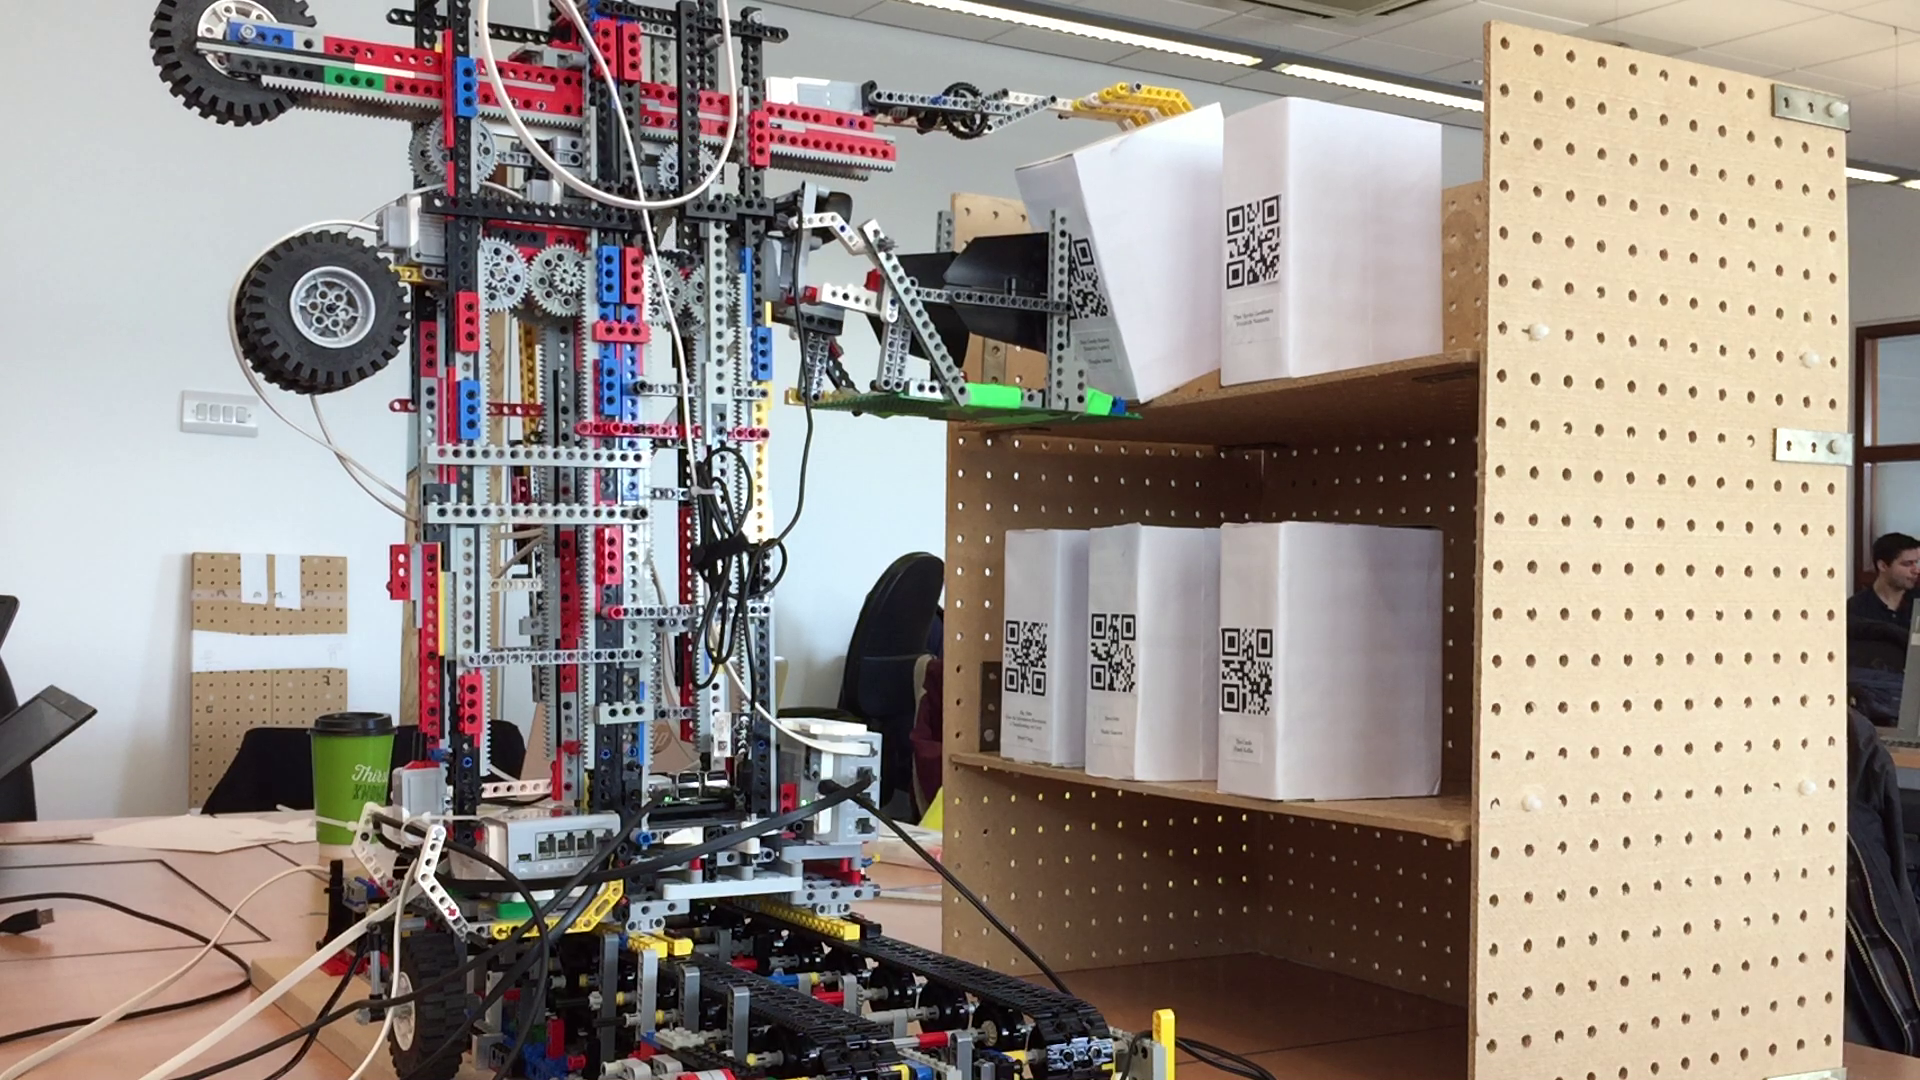
\includegraphics[width=\columnwidth]{figs/crane}}
\caption{Lego construction: highlight any salient features in the caption}
\label{fig:sample-fig}
\end{center}
\vskip -5mm
\end{figure} 


\subsection{Resource distribution}

The 200 hours per member will include the following for every member: {\bf at least} 15-20 hours worth of team meetings, 4 hours of demos with another 4 for preparation, 2 hours of workshops with each member attending at least one, and 1-2 hours for the individual reflection report. This leaves each member with 168 hours to dedicate to their work; roughly 500 hours per team.


\underline{Robot building} 

Our first milestone is to have an early version of the robot base frame built with basic moving functionality in all directions and with a mounted underneath camera to track a pathfinding line of tape. The base should be sturdy and able to hold a medium load. This will take around 100 hours total. The breakdown of this time is: 20 hours of initial design, 40 hours of building, and 20 hours worth of testing.

Sub tasks:

Movement Base Frame
    

The second milestone will take around 40 hours of design, 100 hours of building, and 40 hours of testing. This should be plenty of time to have the final robot designed and ready for milestone 3.

The third milestone will take around 40 hours of designing improvements for the aesthetic and how to add the camera/screen, 20 hours worth of 3D printer work, 20 hours of implementing the improvements, and another 20 hours on testing.

The fourth and final milestone will have all 120 hours dedicated to testing and troubleshooting. The largest amount of time has been allocated to this milestone as it is without a doubt the most critical milestone in the development of the product.

The team will work as a unit at every stage in this with daily subtasks delegated as needed. They will be keeping in close contact with the robot software team and will likely spend a lot of this time working together.

\underline{Robot coding}

Our first milestone is to have the robot move around and follow a tape line.
Sub tasks: 
Basic RC of robot
    Connecting software to motor controls using ROS
    Moving forward and backwards
    Rotating on the spot and turning to face a specified direction angle
    
Robot Pathfinding system
    Internal memory to keep track of the robot's state 
    
    

.140 hours total. That's 25 hours per task, with 10 hours of testing per feature.

Milestone two is to have the robot moving along the line and some light patient interaction. This will take another 140 hours. This will be 100 hours of development on the line following, with 20 hours of testing on this feature, and then 20 hours in the initial development of some basic patient interaction.

The basic connection with the app and the cup holder extension will take 100 hours: 20 hours in the connection, 60 on the holder extension and 20 of testing with the majority of the testing on this phase concentrated on the cup holder extension.

The final 100 hours will be used for the final milestone. 75 of these hours will be on developing the robot path features to work with the app. 25 hours for testing.

\underline{App}

The basic UI design and database setup for milestone one will take around 120 hours. 60 hours of UI design, 30 hours of database setup, and 30 hours to test these two aspects of the app.

Improving the UI and establishing a secure connection with the robot will take a further 100 hours with 60 of these dedicated to the security of the connection, 20 to UI improvement and 20 to test all improvements.

The calendar, alarm, and robot photo features will take another 180 hours. The photo feature will take 70 hours to build and test, the alarm will take 50 to build and test, and the calendar will take 60. The bulk of the work on the app will take place on these 3 complex features.

Polishing up the UI and building potential extensions to the app will be allocated the final 100 hours. This is the point in the development that can be trimmed down if there is more time required for earlier milestones.

\begin{table}[]
  \begin{tabular}{|l|l|l|}
    \hline
    {\bf Team}           & {\bf Member}& {\bf Main skills} \\ \hline
    Project manager      & Michael     & Project management \\ \hline
                         & Jakub       & \\ \cline{2-3}
    Robot building       & Luukas      & \\ \cline{2-3}
                         & Rebecca     & \\ \hline
                         & Ben         & ML/general coding\\ \cline{2-3}
    Robot coding         & Errikos     & Ros/Vis \\ \cline{2-3}
                         & Wojtek      & Ros/Vis \\ \hline
                         & Theo        & \\ \cline{2-3}
    App                  & Yuchen      & \\ \cline{2-3}
                         & Ching Ling  & \\ \hline
  \end{tabular}
  \caption{}
\end{table}

\begin{table}[]
  \begin{tabular}{|l|l|}
    \hline
    {\bf Team}           & {\bf Equipment} \\ \hline
    Robot building       & Turtlebot, Lego, sensors, 3D printer\\ \hline
    Robot coding         & \\ \hline
    App                  & \\ \hline
  \end{tabular}
  \caption{}
\end{table}

\subsection{Risk assessment} 

\underline{Robot building}

One of the risks with the hardware that we identified is the fact that it could be stolen. We addressed this by including an alarm system that will sound if the robot is removed from the area it is expected to be in at any given moment.

\underline{Robot coding}

The main risk to the coding of the robots software is that certain features are not implemented on time. The safeguard to this is that the bulk of the teams time will be used on the essential features with the less important features allocated less time.

\underline{App}

The risk with the app is that the connection is not secure and will be open for attack. Special effort will be put in to this aspect of the product as discussed in Section 2.3.

\section{Group organisation}
\begin{table}[]
  \begin{tabular}{lll}
    \hline
    Robot building & Robot coding & App development   \\
    \hline
    {\bf Jakub}          & {\bf Wojtek}       & {\bf Theo}              \\
    Luukas         & Ben          & Yuchen            \\
    Rebecca        & Errikos      & Ching Ling \\
    \hline
    Project management: & {\bf Michael} & \\
  \end{tabular}
  \caption{Team splits across the group. Names in bold are key points of contact.}
  \label{tab:group-split}
\end{table}

We will split the group into {\bf three core teams}: robot building, robot software, and app development (table~\ref{tab:group-split}). Each team has a team lead (in bold), responsible for co-ordinating with the other groups as necessary during the development process and holding responsibility for ensuring the group is tracking to its milestones.

The project manager (PM) holds overall responsibility for keeping the project on track: primarily through helping each team plan, execute, and validate its progress against milestones. The PM is also responsible for time management; writing up reports; and helping teams with any blockers they encounter in their work.

Structuring the teams in this manner allows us to use the {\it functional} organizational structure. This has particular benefits in allowing everyone within each team to focus on developing expertise in their area, as well as improving efficiency in communication within the team.

The disadvantage of using a functional structure is that it can make communication between teams difficult. To minimize this, we have decided a key point of contact (POC), in bold, for each team: POCs will communicate with each other and the PM on key issues and when cross-team collaboration is needed --- for example, in interfacing the robot hardware with the robot software. This eases communication between teams because it means there will only need to be four people meeting at once to represent all teams, rather than all ten group members needing to be present.

{\bf Each team will meet at a minimum once a week} to discuss their progress against their milestones; however, as demo days approach it will likely move to two or three times a week. Additionally the team POCs will meet once a week to make sure that any cross-team integration issues are handled, as well as to support each other if needed. 

{\bf Code-sharing} will be done exclusively through GitHub. Using version control more generally allows us to track our work over time and easily deal with any merge conflicts or other issues that may come up in doing distributed development. GitHub was chosen primarily because all members of the group are somewhat familiar with it, meaning there will be a shallower learning curve to complete our project using it. 

Using GitHub also allows us to do {\bf task allocation and progress sharing} using GitHub projects. We will follow a Kanban approach, separating tasks into ``to do'', ``in progress'', and ``done'', with one board per team. Using Kanban allows for team members to clearly see what tasks need to be done before the next demo; choose to begin working on tasks they feel they are suitable for; and to identify where there may be blockers within their work (ie. cards that are spending extended time in ``to do''). Additionally, making these boards public allows for other teams to see how work is progressing in the rest of the group. Progress updates will also be discussed in weekly team meetings on a granular level and more broadly in POC meetings.

{\bf Communication} will be done primarily through a dedicated Slack workspace, with separate channels for each team ({\tt robot-app}, {\tt robot-building}, {\tt robot-coding}, {\tt report-writing}, and {\tt general} for cross-team discussion). Using Slack allows us to integrate other apps, for example Doodle polls to decide group meeting times; and GitHub to track push or other notifications from our project repository. 


%% Include any references in a bibliography

\bibliography{plan-refs}

\end{document} 

